O retificador trifásico de onda completa utiliza uma ponte de Graetz, como já vimos. A figura \ref{ctcl} ilustra o circuito.

\begin{figure}[h]
\center
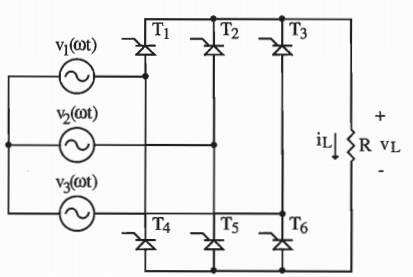
\includegraphics[scale=0.55]{imagens/circuito_trifasico_onda_completa.png}
\caption{Circuito do retificador trifásico de onda completa.} \label{ctcl} 
\caption*{Fonte: Eletrônica de potência (2006)}
\end{figure}

No caso da carga puramente resistiva, temos, primeiro, a situação do ângulo de disparo $\alpha = 0$, no qual é fácil ver que \[
V_{L,med} \approx 2,34 V_o
\] como já vimos para o caso equivalente implementado a diodo.

Já para $0<\alpha <\frac{\pi}{3}$, ainda há condução contínua e a tensão média na carga é 
\begin{align*}
    V_{L,med} &= \frac{6}{2\pi}\int_{\frac{\pi}{3}+\alpha}^{\frac{2\pi}{3}+\alpha}\sqrt{2}V_{OL}\sin(\omega{t})d(\omega{t})\\
	      &= \frac{6\sqrt{2}V_{OL}}{2\pi}\left[-\cos\left(\frac{2\pi}{3}+\alpha\right) + \cos\left(\frac{\pi}{3}+\alpha\right)\right] \\
    &= \frac{6\sqrt{2}V_{OL}}{2\pi}\cos\alpha\\
    &\approx 1,35V_{OL}\cos\alpha\\
    V_{OL} &= \sqrt{3}V_{o} \approx 1,73V_{o}\\
    \implies V_{L,med} &\approx 2,34V_{0}\cos\alpha
.\end{align*}

Para o caso da condução descontínua, i.e., $\frac{\pi}{3}<\alpha<\frac{2\pi}{3}$, a tensão média se torna
\begin{align*}
    V_{L,med} &= \frac{6}{2\pi}\int_{\frac{\pi}{3}+\alpha}^{\pi}\sqrt{2}V_{OL}\sin(\omega{t})d(\omega{t})\\
&\approx 2,34V_{o}\left[1 + \cos\left(\frac{\pi}{3}+\alpha \right)\right]
.\end{align*}

A relação entre a tensão média na carga e o ângulo de disparo pode ser observada na figura \ref{g1tcr}.

\begin{figure}[h]
\center
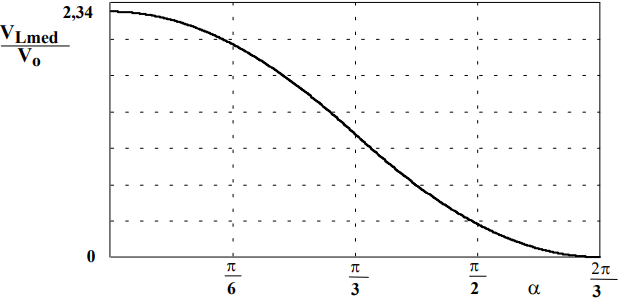
\includegraphics[scale=0.55]{imagens/grafico1_trifasico_onda_completa_r.png}
\caption{Tensão média na carga puramente resistiva de um retificador trifásico de onda completa a tiristor.} \label{g1tcr} 
\caption*{Fonte: Eletrônica de potência (2006)}
\end{figure}

Ambos os casos de condução são ilustrados na figura \ref{g1tcl}.

\begin{figure}[h]
\center
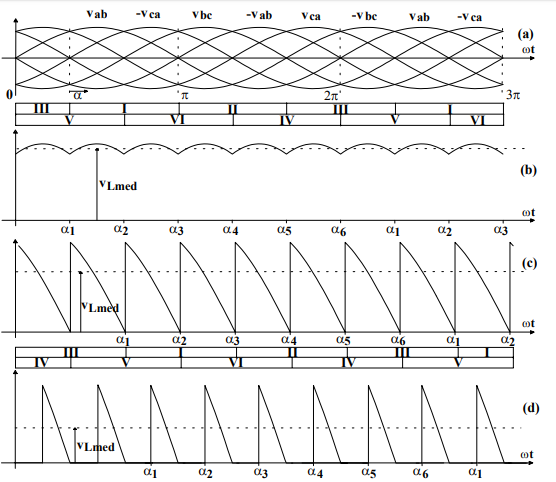
\includegraphics[scale=0.55]{imagens/grafico1_trifasico_onda_completa_l.png}
\caption{(a) Tensões de linha da rede. (b) Tensão na carga para $\alpha =0$. (c) Tensão na carga para $\alpha = \frac{\pi}{3}$. (d) Tensão na carga para $\alpha>\frac{\pi}{3}$ .} \label{g1tcl} 
\caption*{Fonte: Eletrônica de potência (2006)}
\end{figure}

Para uma carga com componente indutivo, a figura \ref{g2tcl} ilustra o comportamento da tensão na carga.

\begin{figure}[h]
\center
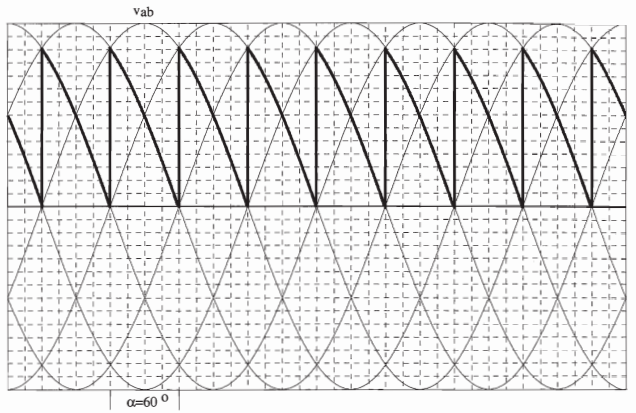
\includegraphics[width=0.45\textwidth]{imagens/grafico2_trifasico_onda_completa_l.png}
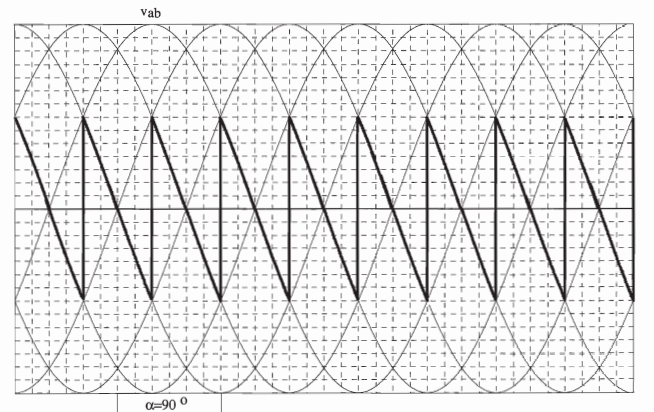
\includegraphics[width=0.45\textwidth]{imagens/grafico3_trifasico_onda_completa_l.png}
\caption{Tensão na carga com componente indutivo em um retificador trifásico de onda completa a tiristor.} \label{g2tcl} 
\caption*{Fonte: Eletrônica de potência (2006)}
\end{figure}

Nesse caso, a tensão média na carga é
\begin{align*}
    V_{L,med} &= \frac{3}{\pi}\int_{\frac{\pi}{3}+\alpha}^{\frac{2\pi}{3}+\alpha}\sqrt{2}V_{OL}\sin(\omega{t})d(\omega{t})\\
	      &= \frac{3\sqrt{2}V_{OL}}{\pi}\left[-\cos\left(\frac{2\pi}{3}+\alpha\right) +\cos\left(\frac{\pi}{3}+\alpha\right) \right] \\
&\approx 1,35V_{OL}\cos(\alpha)\\
&\approx 2,34V_{o}\cos(\alpha)
.\end{align*}

Dessa forma, é fácil ver que o circuito opera como um retificador para $0<\alpha<\frac{\pi}{2}$ e como um inversor não autônomo para $\frac{\pi}{2}<\alpha<\pi$.


